\section{BB84}
  \index{BB84}
  \rhead{BB84}
  \subsection{Das BB84 Protokoll}
  Das BB84 Protokoll, wurde 1984 von Charles H. Bennett and Gilles Brassard entwickelt,
  was auch den Namen des Protokolls gepr\"agt hat.
  Es war das erste Protokoll, welches es erm\"oglichte eine \"Ubertragung \"uber zwei unsichere Kan\"ale zu f\"uhren
  und dabei lauschende Dritte eindeutig zu erkennen und dennoch einen sicheren Schl\"ussel zu \"ubertragen.

  \subsection{Ohne Lauscher}
  Die verschl\"usselte Kommunikation soll zwischen Alice und Bob stattfinden.
  F\"ur das BB84 Protokoll sind zwei Kommunikationskan\"ale n\"otig:
  Ein konventioneller, sowie ein Quantenkanal, oft wird daf\"ur ein optisches Medium verwendet.
  Alice beginnt polarisierte Photonen zu erstellen und \"uber das optische Medium an Bob zu senden.
  Dabei verwendet sie eine der zwei um $45^{\circ}$ verdrehte Basen,
  welche jeweils zwei um $90^{\circ}$ verdrehte Polarisierungen aufweisen und damit die Werte 1 und 0 repr\"asentieren. Siehe Abbildung \ref{crypto:poltab}

  \begin{figure}
    \centering
    \begin{tabular}{l l || c c}
      \hline
      $(+)$ & rectilinear & $(\uparrow)$ & $(\rightarrow)$\\
      $(\times)$ & diagonal & $(\nearrow)$ & $(\searrow)$\\
      \hline
      & & $0$ & $1$\\
      \hline
    \end{tabular}
    \caption{Die Polarisierungen der Photonen und ihre Bedeutung\label{crypto:poltab}}
  \end{figure}

  Die polarisierten Photonen dienen also als Qubits, das Quanten\"aquivalent eines konventionellen Bits.
  Dabei muss sich Alice die Reihenfolge der verwendeten Basen merken,
  denn sie werden sp\"ater ben\"otigt um eine statistische Analyse der \"Ubertragungsfehler zu erstellen.

  Bob nimmt die polarisierten Photonen entgegen und w\"ahlt zuf\"allig eine der beiden Basen aus durch welche er das Photon analysiert.
  Dabei w\"ahlt Bob mit
  $P(\text{richtig})=0.5$
  die richtige Basis.
  W\"ahlt Bob die falsche Basis erh\"alt er mit
  $P(\text{korrekt}|\text{falsch})=0.5$
  das korrekte Resultat, bei
  $P(\text{korrekt}|\text{richtig})=1$
  f\"ur das korrekte Resultat bei der richtigen Basis ergibt das ein
  $P(\text{korrekt})=0.75$,
  dass ein Photon korrekt gemessen wurde.
  Siehe Abbildung \ref{crypto:BB84KE}

  Nachdem gen\"ugend Photonen gesendet wurden, um einen ausreichend starken symmetrischen Schl\"ussel zu erzeugen, findet zwischen Alice und Bob die sogenannte Basendiskussion statt.
  Dazu sendet Bob die Information, welche Basis er f\"ur welches Photon verwendet hat, \"uber den konventionellen Kanal zu Alice.
  Alice meldet ihm, bei bei welchen Photonen er die richtige Basis, also dieselbe, welche auch sie f\"ur die Polarisation verwandte, verwendet hat.
  Zur \"Uberpr\"ufung ob die Verbindung belauscht wurde, f\"uhren Alice und Bob eine statistische Analyse der Verteilung der \"Ubertragungsfehler aus.
  Wenn die Verbindung nicht manipuliert wurde, ist mit $P(\text{korrekt})=0.75$ zu rechnen.
  F\"ur Detail siehe Abbildung \ref{crypto:bittab}

  \begin{figure}
    \centering
      \begin{tabular}{ l || c | c | c | c | c | c | c | r }
        \hline
        A's Zufallsbits & 0 &  1 & 1 & 0 & 1 & 0 & 0 & 1 \\
        \hline
        A's Basen & $+$ & $+$ & $\times $ & $+$ & $\times $ & $\times $ & $\times $ & $+$ \\
        \hline
        A's Polarisation & $\uparrow$ & $\rightarrow$ & $\searrow$ & $\uparrow$ & $\searrow$ & $\nearrow$ & $\nearrow$ & $\rightarrow$ \\
        \hline
        B's Basen & $+$ & $+$ & $\times $ & $\times $ & $+$ & $\times $ & $+$ & $+$ \\
        \hline
        B's Polarisation & $\uparrow$ & $\rightarrow$ & $\searrow$ & $\nearrow$ & $\rightarrow$ & $\nearrow$ & $\rightarrow$ & $\rightarrow$ \\
        \hline
        B's gemessene Bits & 0 & 1 & 1 & 0 & 1 & 0 & 1 & 1 \\
        \hline
        Decoypuls & & \checkmark & & & & & \checkmark & \\
        \hline
        Basen Diskussion \\
        \hline
        Shared Key Bits& 0 & & 1 & & & 0 & & 1 \\
        \hline
      \end{tabular}
      \caption{Auswertung der Polarisation und der Status\label{crypto:bittab}}
  \end{figure}

  \begin{figure}
    \centering
    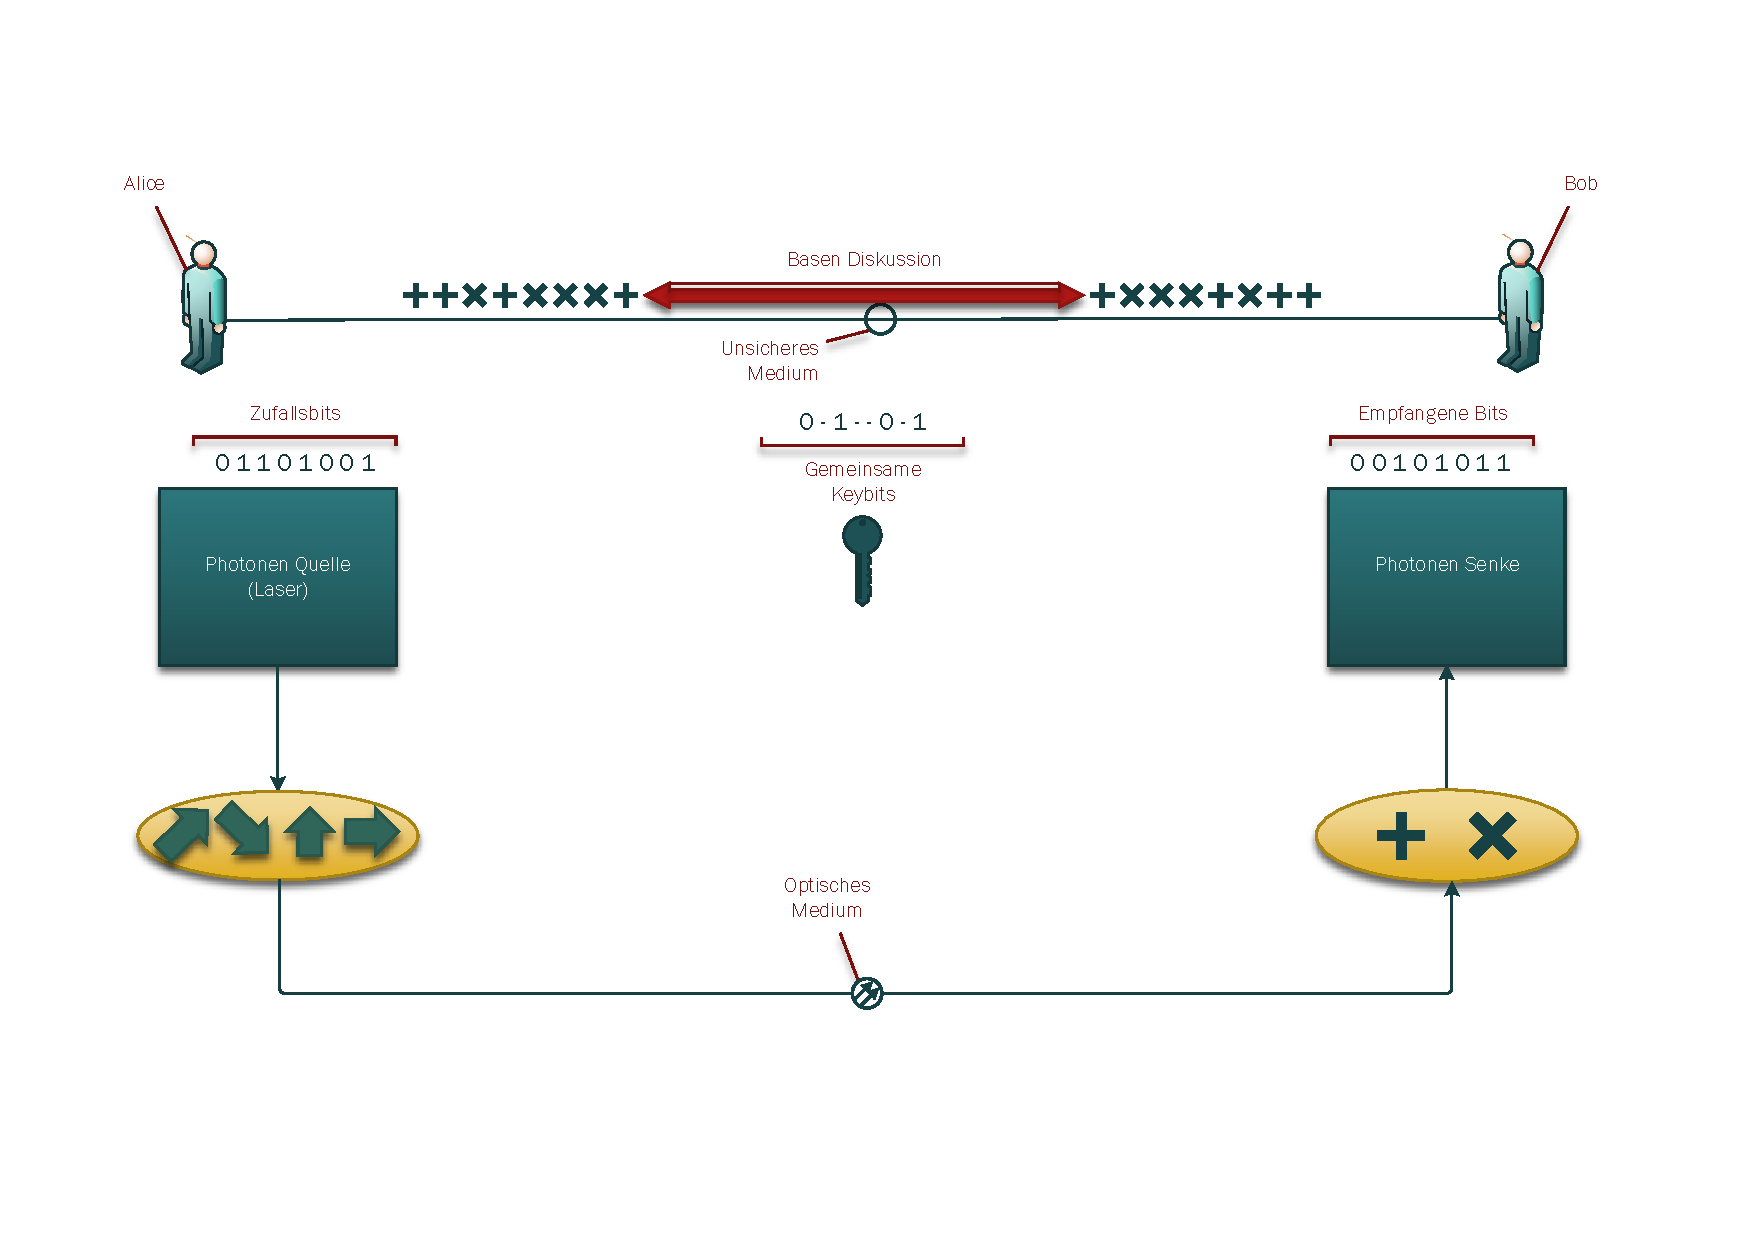
\includegraphics[height=0.45\textheight]{crypto/BB84.pdf}
    \caption{Normalfall des Schl\"usselaustausches mit BB84\label{crypto:BB84KE}}
  \end{figure}

  \subsection{Mit Lauscher}
  Das BB84 Protokoll erm\"oglicht es, einen Lauscher (Eavesdropper) zu bemerken.
  In konventionellen Schl\"usselaustausch Protokollen z.B.(DH, ECDH)
  beruht die Sicherheit des Schl\"ussels auf der mathematischen Komplexit\"at.
  Einem Lauscher ist es also m\"oglich den Schl\"ussel zu errechnen,
  wenn er nur einen ausreichend leistungsf\"ahigen Rechner hat.

  Beim BB84 Protokoll kann ein Lauscher jedoch nicht lauschen, ohne die \"Ubertragung zu beinflussen.
  Doch warum? Was \"andert sich wenn Eve lauscht? Siehe Abbildung \ref{crypto:BB84Eve}
  Eve f\"angt die von Alice polarisierten Photonen ab und misst sie mit 50\% Wahrscheinlichkeit korrekt.
  $P(\times)=0.5, P(+)=0.5$
  Danach generiert Eve ein neues Photon, mit derselben Polarisation,
  wie die, welche sie gemessen hat und sendet es weiter zu Bob.
  Da Eve auch nur mit
  $P(\text{korrekt})=0.75$
  korrekt misst, kann sie auch nur in
  $75\%$
  der F\"alle die richtige Polarisation erzeugen.
  Bob kann also nur noch mit
  $P(\text{korrekt}|\text{Eavesdropper})=0.75\cdot 0.75=0.625$
  die korrekte Polarisation messen.
  Um dies festzustellen tauschen Alice und Bob einige Schl\"usselbits aus.
  Dazu werden sogenannte Decoypulses eingebaut, das sind Bits,
  welche nur f\"ur die Statistik dienen und nicht im Schl\"ussel Verwendung finden.

  \begin{figure}
    \centering
    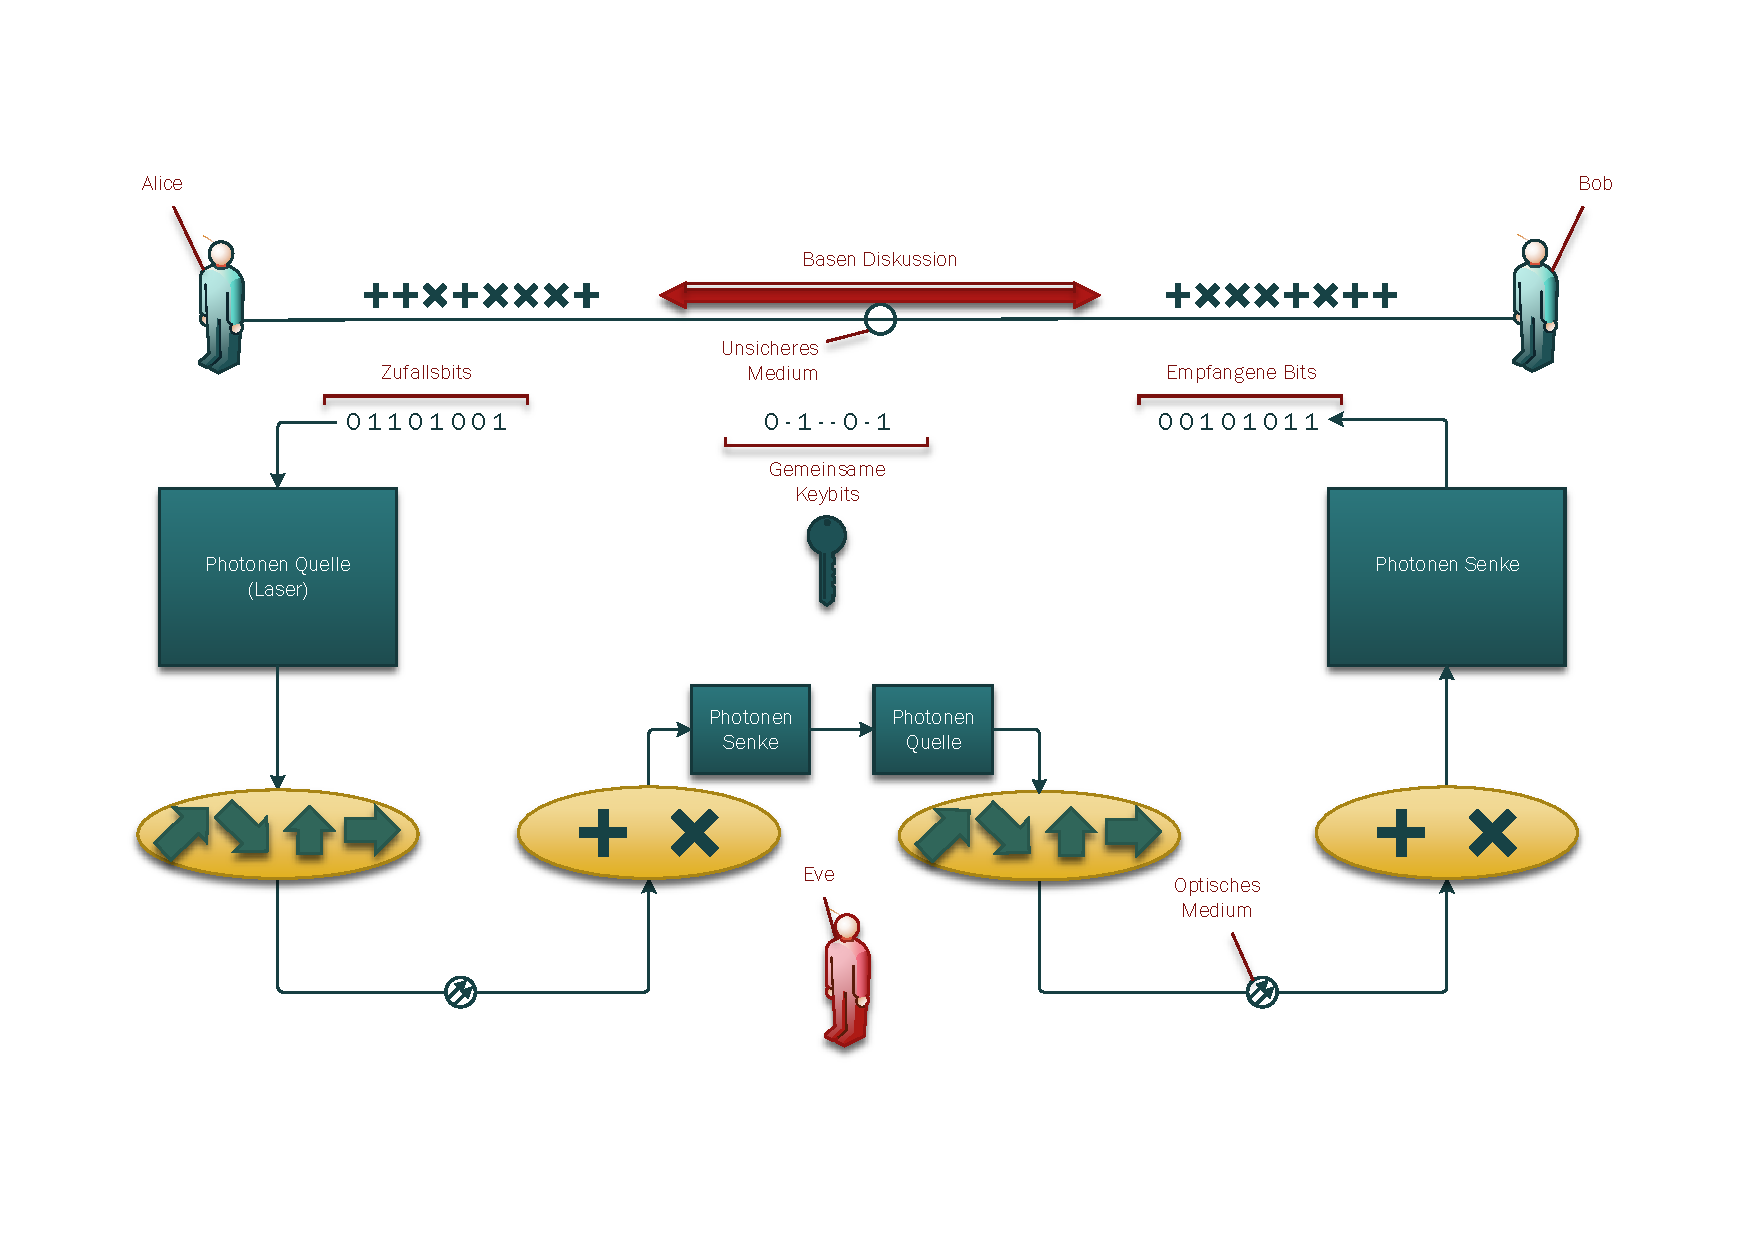
\includegraphics[height=0.45\textheight]{crypto/BB84Eve.pdf}
    \caption{Schl\"usselaustausch mit Eavesdropper\label{crypto:BB84Eve}}
  \end{figure}

  Die einzige m\"ogliche Art von Eavesdropping ist, wenn Eve bei der Quelle die M\"oglichkeit hat, \"uberz\"ahlige Photonen abzuzweigen,
  sie zu lagern und nachdem Alice und Bob die Basendiskussion gef\"uhrt haben,
  mit dem der richtigen Basis zu messen und dadurch einzelne g\"ultige Keybits zu erhalten.

  \subsection{No-Cloning}
  Die Grundlage f\"ur das Funktionieren dieser Methode bietet die Tatsache, dass man nicht beliebige Zust\"ande auf einen anderen kopieren kann, siehe No-Cloning-Theorem (NCT \ref{skript:no-cloning-theorem}).
  Eve kann aufgrund des No-Cloning-Theorems die Photonen von Alice nicht einfach kopieren und die Kopie an Bob schicken,
  sondern ist gezwungen anhand ihrer Messungen (von denen h\"ochstens 75\% korrekt sind) selbst Photonen zu polarisieren
  und Bob zu senden, was bei Bob zu einer Trefferrate von weniger als 0.75 f\"uhrt.
  $P(\text{korrekt}|\text{Eavesdropper})<0.75$

  Wenn man also Eve mit $P=0.999999999$ aufsp\"uren will,
  folgt aus $P_d = 1 - \left(\frac{3}{4}\right)^n$,
  dass 72 Keybits ausgetauscht werden m\"ussen.

  Da es so etwas wie einen Photonen-Kopierer nicht gibt, ist ein Scenario mit undetektierbarem Lauschen nicht m\"oglich (Abbildung \ref{crypto:BB84Clone}).

  \begin{figure}
    \centering
    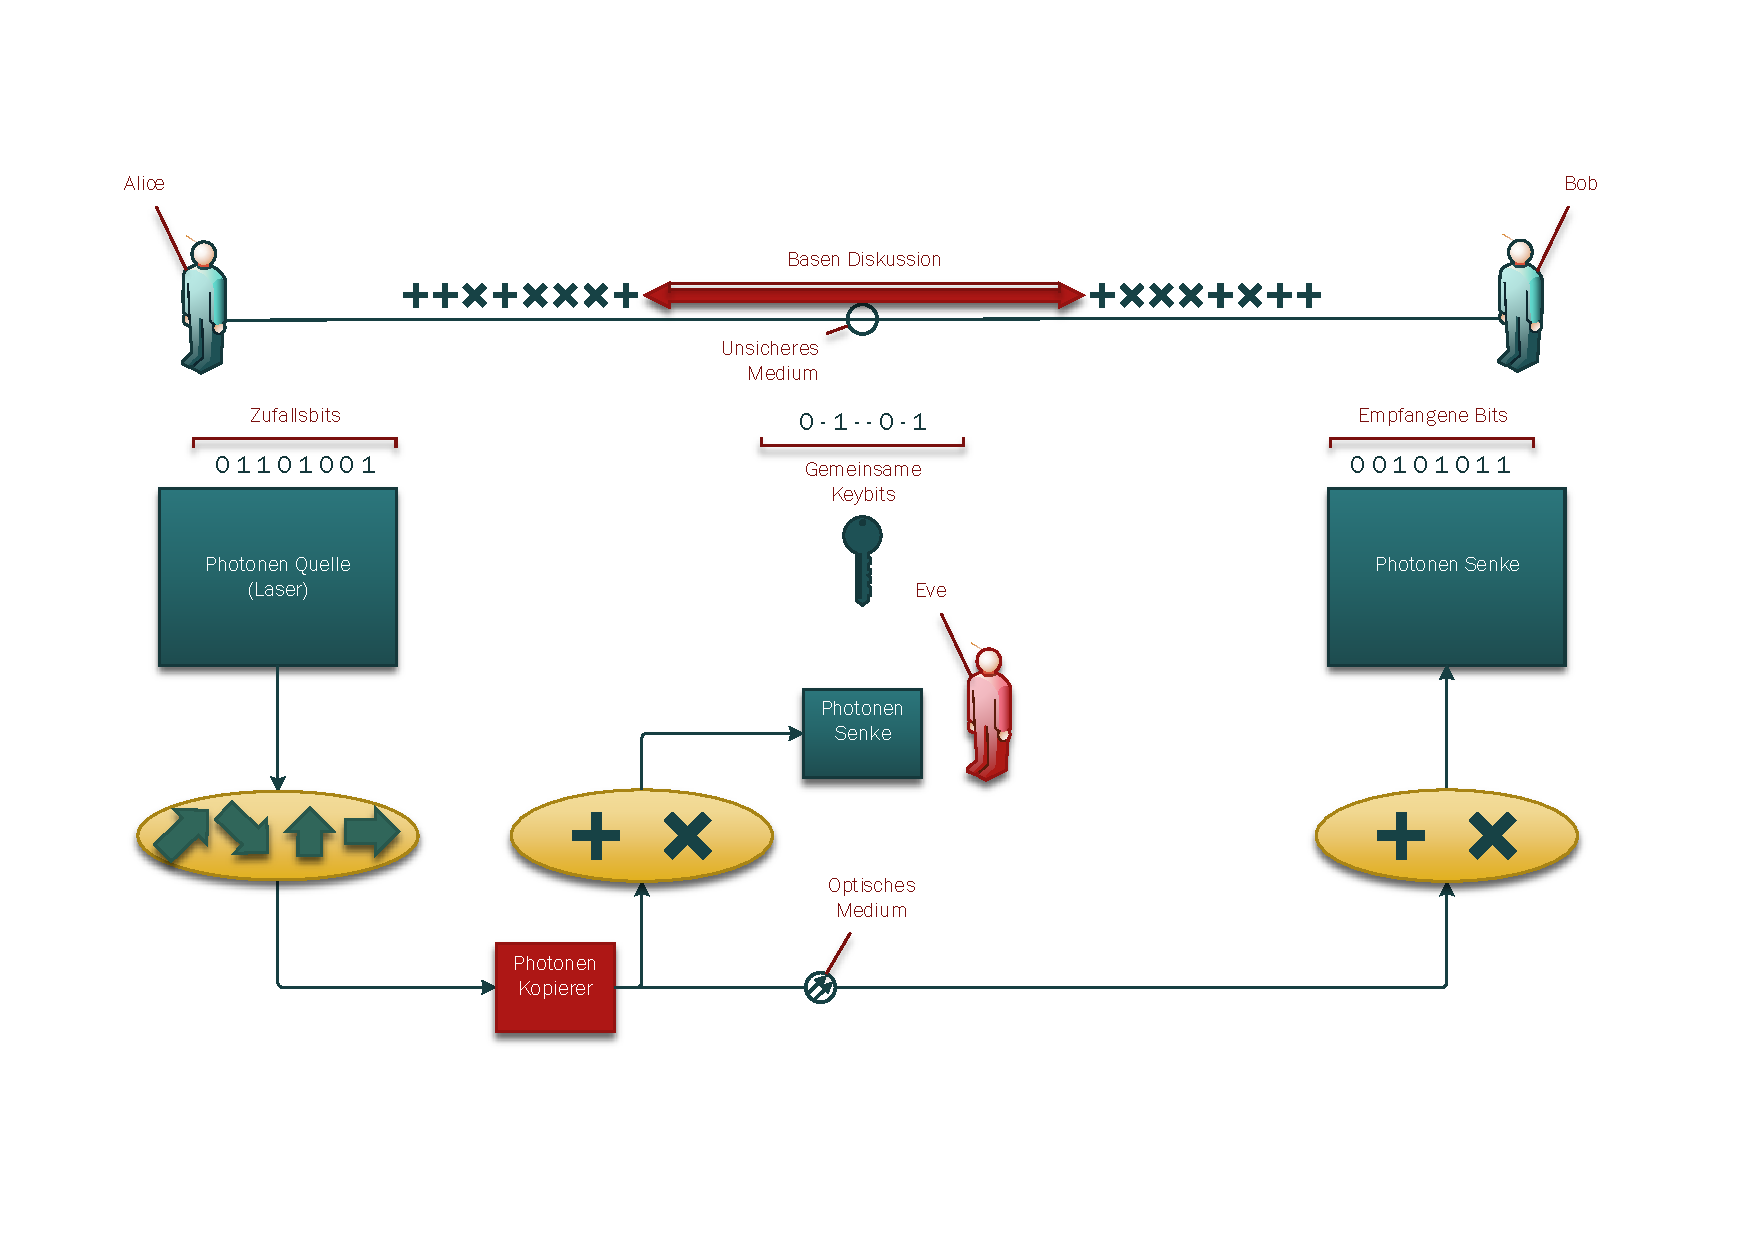
\includegraphics[height=0.45\textheight]{crypto/BB84Eve-Clone.pdf}
    \caption{Theoretischer Einsatz des Photonen-Kopierers\label{crypto:BB84Clone}}
  \end{figure}

  \subsection{Schw\"achen}
  Es gibt Angriffe welche mittels Blendung des Detektors die \"Ubertragung des Schl\"ussels belauschen
  und dabei undetektierbar bleiben. \cite{qc:detector}

  Zudem sch\"utzt das BB84 Protokoll nicht vor einer Man in the Middle Attacke (Siehe Abbildung \ref{crypto:BB84Max}),
  jedoch kann diese vermieden werden, indem eine Authentisierung des Partners verwendet wird.
  Dies ist auch mittels quantenmechanischer Effekten realisierbar. \cite{qc:Authentisierung}

  \begin{figure}
    \centering
    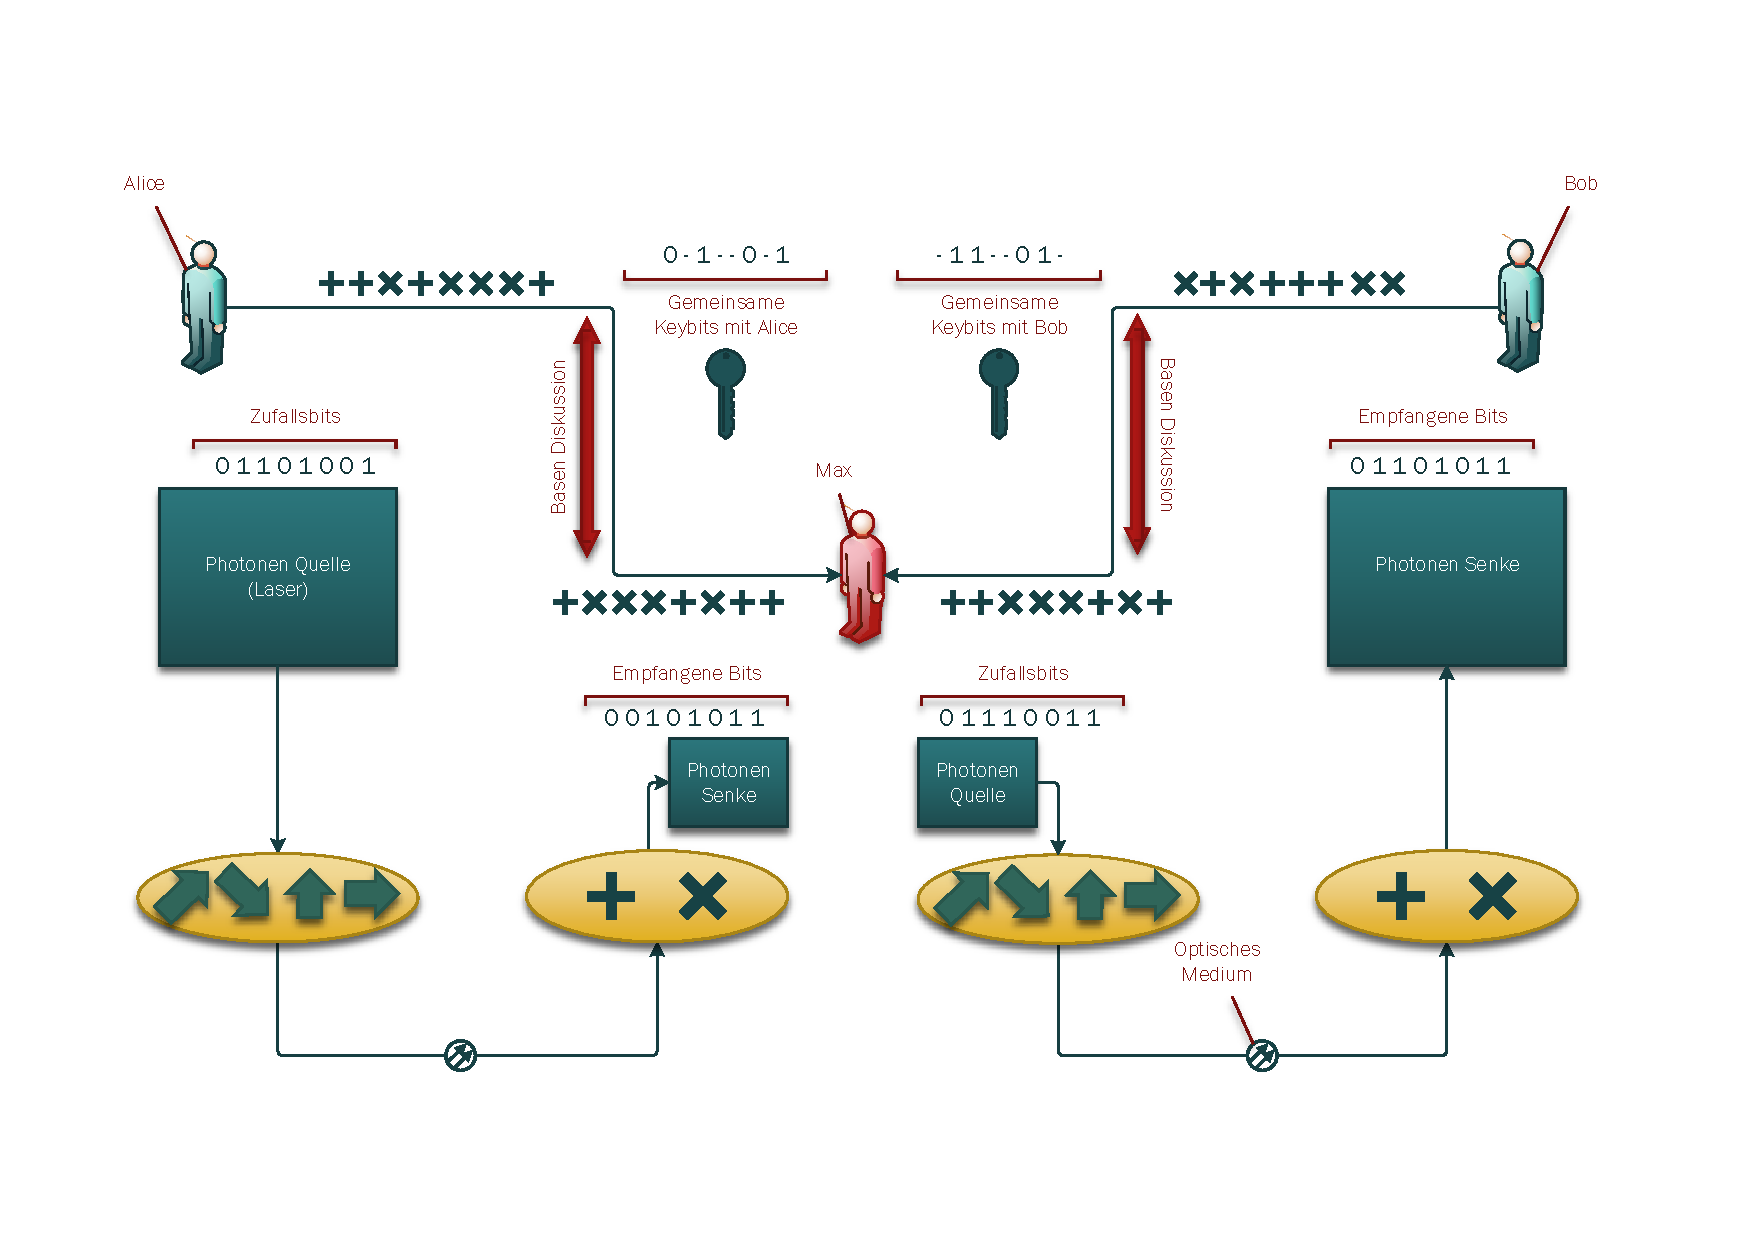
\includegraphics[height=0.45\textheight]{crypto/BB84Max.pdf}
    \caption{Austausch mit Max als Man in the Middle\label{crypto:BB84Max}}
  \end{figure}
